\chapter{Ongelmat JavaScriptin staattisessa tyypittämisessä}

\section{EcmaScript-yhteensopivuus}
TypeScript pyrkii noudattamaan EcmaScript-spesifikaatiota mahdollisimman
tarkasti kaikkien sellaisten ominaisuuksien suhteen jotka eivät nimenomaan
liity staattiseen tyypittämiseen \cite{TypeScript_DesignGoals}. TypeScriptin
kehityksen alkuvaiheissa, ennen EcmaScript 2015-spesifikaation valmistumista,
JavaScriptista kuitenkin puuttui joitain tärkeiksi katsottuja ominaisuuksia,
jotka päätettiin lisätätä TypeScriptiin mahdollisista yhteensopimusongelmista
huolimatta. TypeScriptissä on esimerkiksi syntaksi nimiavaruuden määrittämiseen,
vaikka EcmaScriptiin myöhemmin lisätyt \textit{moduulit} ajavat saman asian
\cite{TypeScript_issuecomment_esnextfeatures}. TypeScript tukee nykyään sekä
alkuperäistä nimiavaruus-ominaisuuttaan että EcmaScriptin moduuleita.

Flow ja Closure-kääntäjä lisäävät koodiin ainoastaan staattista tyypitystä
koskevia ominaisuuksia, kuten tyyppimäärittelyjä, joten niissä ei ole
nimiavaruuksien kaltaisia koodin suoritukseen vaikuttavia ominaisuuksia.
EcmaScript kuitenkin kehittyy nopeasti ja sen päälle rakentavien työkalujen
on pysyttävä tahdissa mukana ollakseen hyödyllisiä kehittäjille.

Kaikki kolme työkalua pyrkivät tukemaan EcmaScriptin uusinta viimeisteltyä
versiota. Lisäksi Flow tarjoaa tyyppitarkastusta joillekkin kokeellisille
ominaisuuksille joiden EcmaScript-määrittely ei vielä ole täysin valmis mutta
jotka luultavasti tullaan lisäämään myöhemmin. Esimerkiksi
\textit{null-turvallinen ketjutus} (engl. optional chaining tai safe navigation)
\cite{Optional_Chaining_proposal} on vielä
suunnitteluvaiheessa oleva kielen ominaisuus, mutta Flow tarjoaa jo
staattisen tyyppitarkastuksen sille. Uusien ominaisuuksien aikaisessa
käyttöönotossa on JavaScriptin kehityksen kannalta se hyvä puoli, että
kehittäjäyhteisö pääsee kokeilemaan ja antamaan palautetta ennen kuin ominaisuuden
määrittely on lyöty lukkoon. TypeScript puolestaan pyrkii vastedes implementoimaan
ainoastaan valmiita ominaisuuksia, sillä keskeneräisen ominaisuuden yksityiskohdat
tulevat suurella todennäköisyydellä muuttumaan useaan otteeseen suunnitteluvaiheen
aikana ja sitä käyttäneet kehittäjät voivat myöhemmin joutua
\textit{refaktoroimaan} koodiaan.

\section{Tyyppien automaattinen ja vaiheittainen tyypittäminen}

Jotta staattisen tyypityksen tuova työkalu olisi varteenotettava vaihtoehto
dynaamisesti tyypitetyn JavaScriptin rinnalla, sen kirjoittaminen ei voi vaatia
liian paljon enemmän työtä kuin JavaScriptin. Staattisessa tyyppijärjestelmässä
näkyvin ero dynaamisesti tyypitettyyn on eksplisiittiset tyyppiannotaatiot,
jotka voivat olla lisärasite koodin kirjoittajalle. Erityisesti vanhaa,
dynaamisesti tyypitettyä JavaScriptia refaktoroidessa staattisesti tyypitettyyn
muotoon on kätevää jos jokaista muuttujaa ja funktiota ei tarvitse muokata
uuteen kieleen siirryttäessä.

TypeScript, Flow ja Cosure-kääntäjä tukevat melko pitkälle kehittynyttä
tyyppien automaattista päättelyä (engl. type inference).
\begin{lstlisting}[caption={
  Flow pystyy tulkitsemaan vertaaHintoja-funktion tyypin automaattisesti, ilman eksplisiittisiä tyyppimäärittelyitä.
  },
  label={fig:flow_call_site_inference},
  aboveskip={20pt}
]
  const vertaaHintoja = (a, b) => a.hinta - b.hinta;
  tuotteet.sort(vertaaHintoja);
\end{lstlisting}
Esimerkissä \ref{fig:flow_call_site_inference}, Flow pystyy päättelemään
tyypin \newline
\inlinecode{vertaaHintoja: (a: Ostos, b: Ostos) => number} automaattisesti,
vaikkei esimerkissä ole yhtään eksplisiittistä tyyppimäärittelyä tai
muuta tavallisesta JavaScriptista poikkeavaa. Flow tietää ennestään
mikä listan sort-metodin tyyppi on, joten se pystyy päättelemään myös
sort-metodille annetun vertaaHintoja-funktion tyypin käyttämällä
\textit{kutsumispaikkaan perustuvaa päättelyä} (engl. call-site inference).
TypeScript ei tue kutsumispaikkaan perustuvaa päättelyä samalla tavalla kuin
Flow, mikä onkin yksi isoimmista eroista näiden kahden työkalun välillä.
Liian pitkälle viety tyyppien automaattinen päättely voi johtaa ongelmiin
sekavien virheviestien tai työkalun hitauden muodossa, minkä vuoksi TypeScript
vaatii nimettyjen funktioiden argumenteille aina eksplisiittiset tyypit.
Kun funktion signatuuriin lisätään \inlinecode{(a: Ostos, b: Ostos)},
myös TypeScript pystyy automaattisesti päättelemään että funktion palautusarvo
on numero, eikä eksplisiittistä \inlinecode{: number} palautusarvon
määritystä tarvita.
Molempien työkalujen tapauksessa on hyvä huomata että tyyppien automaattinen
päättely on viety paljon pidemmälle kuin se funktion sisäinen muuttujan
tyypin päättely jollaista nähdään esimerkiksi
\inlinecode{var}-avainsanalla C\#:issa ja Javassa.

\section{Luotettavuus, täydellisyys ja käytännöllisyys}
\begin{figure}[!htb]
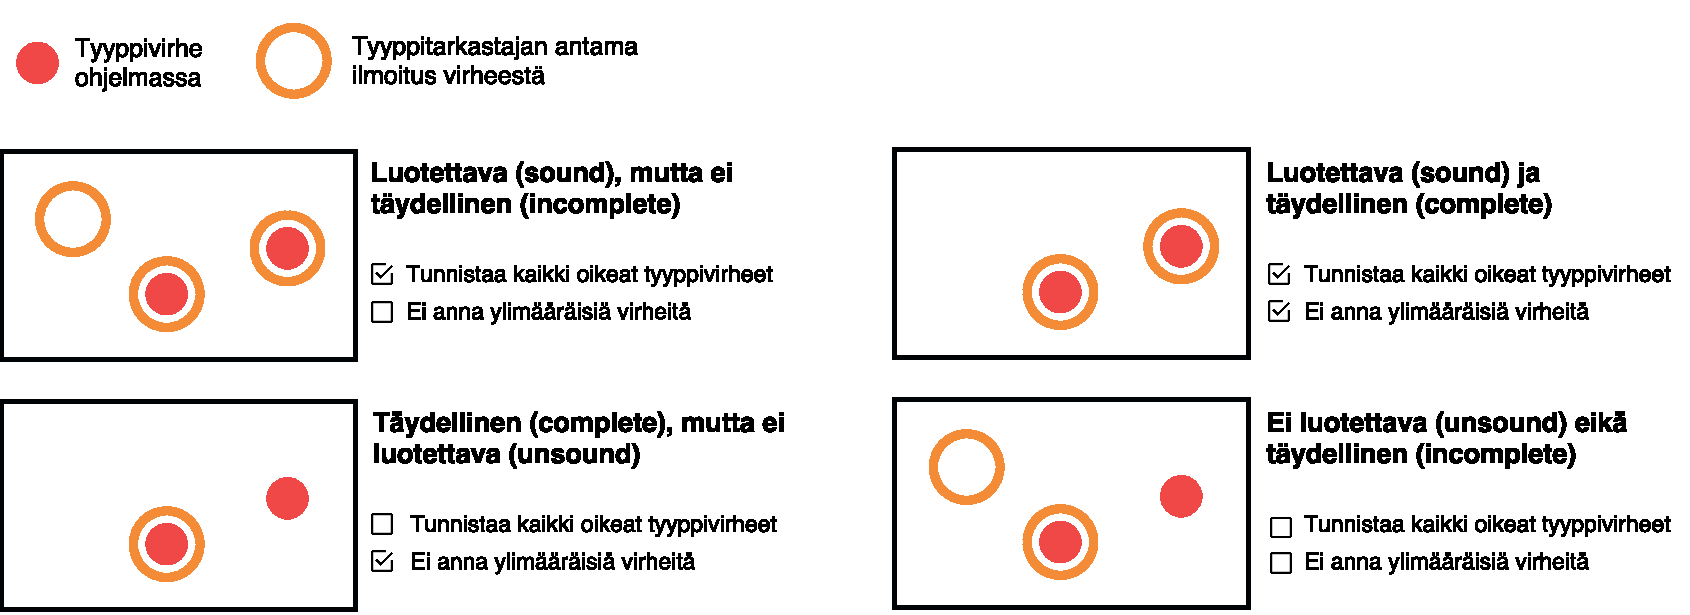
\includegraphics[width=\textwidth]{images/soundness_completeness2.pdf}
\caption{Tyyppijärjestelmän luotettavuus ja täydellisyys}
\end{figure}
Tyyppijärjestelmän luotettavuus (engl. soundness) kuvaa sitä, kuinka suuren osan
mahdollisista ohjelmointivirheistä se estää. Täysin luotettava (engl. sound)
tyyppijärjestelmä estää kaikki sellaiset virheet jotka sen on tarkoitus
estää \cite{CSE_ProgrammingLanguages}. Täydellisyys (engl. \mbox{completeness})
puolestaan kertoo salliiko tyyppijärjestelmä kielen sellaiset ominaisuudet
jotka eivät olisi ajonaikana tyyppivirheitä \cite{TypesAndProgrammingLanguages, CSE_ProgrammingLanguages}.

Jotta JavaScriptiä analysoiva tyyppijärjestelmä olisi luotettava, sen on
annettava virhe esimerkiksi seuraavasta ohjelmasta:

\begin{lstlisting}[caption={Virheellinen JavaScript-ohjelma: lisätyllä tuotteella ei ole nimeä.},label={fig:soundness_test}]
function osta(ostos) {
  lisääTuote({
    nimi: ostos.nimi,
    hinta: ostos.hinta
  });
}

osta({ nimi: 'juusto', hinta: 5 });
osta({ hinta: 5 });
\end{lstlisting}
Toisaalta jotta JavaScriptiä analysoiva tyyppijärjestelmä olisi täydellinen,
sen on sallittava tämä korjattu versio ylläolevasta ohjelmasta:
\begin{lstlisting}[caption={Toimiva JavaScript-ohjelma: virheelliseltä kutsulta on suojauduttu tarkistuksella.},label={fig:completeness_test}]
function osta(ostos) {
  if (typeof ostos.nimi === 'string') {
    lisääTuote({
      nimi: ostos.nimi,
      hinta: ostos.hinta
    });
  }
}

osta({ nimi: 'juusto', hinta: 5 });
osta({ hinta: 5 });
\end{lstlisting}
Esimerkit \ref{fig:soundness_test} ja \ref{fig:completeness_test} toimivat
odotetulla tavalla Flow:ssa. TypeScript vaatii eksplisiittisen tyyppiannotaation
osta-funktiolle, mutta toimii muuten samalla tavalla. Flow, TypeScript ja
Closure eivät kuitenkaan ole täydellisiä tai kokonaan luotettavia.
Monimutkaisemmissa tilanteissa virheitä saattaa jäädä nappaamatta tai toimiva
ohjelma voidaan merkata virheelliseksi.

JavaScriptiä käännöskohteena käyttävät
mutta muuten sen syntaksista ja semantiikasta eroavat uudet kielet,
kuten Dart, Elm ja ReasonML on voitu kehittää toivotunlaiseksi ilman painetta olla
yhteensopiva vanhan koodin kanssa. TypeScript ja Flow on sen sijaan kehitetty
lisäämään staattinen tyypitys olemassa olevaan kieleen, JavaScriptiin,
siten että nykyisellään käytössä olevat kirjastot ja koodikäytännöt pystytään
tyyppitarkastamaan ilman että niiden arkkitehtuuria tarvitsee merkittävästi
muuttaa tyyppiturvallisuuden saavuttamiskesi.

TypeScriptin tyyppijärjestelmä on \textit{rakennepohjainen} (engl. structural),
koska sen katsottiin sopivan paremmin siihen tyyliin jolla JavaScriptiä tavallisesti
käytetään. Rakennepohjaisessa tyyppijärjestelmässä keskitytään objektien muotoon
eikä \textit{nimelliseen} (engl. nominal) arvoon, minkä vuoksi myös seuraava koodi kääntyy
ilman tyyppivirheitä.

\begin{lstlisting}[caption={
  Loogisen virheen sisältävä, mutta ilman varoituksia kääntyvä TypeScript-ohjelma.
}, label={fig:structural_typing_error}]
class Ihminen {
    constructor(public nimi: string){}
}
class Eläin {
    constructor(public nimi: string){}
}
function varaaEläinlääkäri(omistaja: Ihminen, lemmikki: Eläin){}

varaaEläinlääkäri(new Eläin("Musti"), new Ihminen("Jaakko"));
\end{lstlisting}
TypeScript-kääntäjä sallii esimerkin \ref{fig:structural_typing_error} koodin
vaikka arugmentit \mbox{\dblquoted{omistaja}} ja \mbox{\dblquoted{lemmikki}}
ovat väärin päin, sillä molempien luokkien rakenne on sama; molemmissa on
pelkkä tekstimuotoinen ominaisuus \dblquoted{nimi}. Flow:ssa sama virhe ei menisi läpi.
Siinä luokkainstanssit on tyypitetty nominaalisesti, mikä auttaa tässä
esimerkissä mutta aiehuttaa ongelmia muissa tilanteissa. Projekti saattaa
esimerkiksi sisältää kaksi versiota samasta kirjastosta jonkin toisen
kirjaston kautta, mikä voi aiheuttaa yhteensopimusongelmia kun käytännössä
saman luokan tyyppejä ei lueta keskenään yhteensopiviksi.